\documentclass[esd, manuscript]{copernicus} % uncomment to see what the 2 column final paper will look like.

\begin{document}

\section{The emulator}

We treat the output of the simulator (y) as an uncertain function f() of the simulator inputs x, so that y = f(x). We wish to produce a predictive distribution for Y = f(x) at any model input, conditional on the points already run, or the design X. Throughout the study, we use a kriging function, similar to a Gaussian process regression emulator, as coded in the R package DiceKriging \citep{roustant2012dicekriging} for prediction of climate simulator output at untried inputs.
The kriging model or Gaussian Process regression is specified hierarchically with a separate mean and covariance function. For prediction purposes, we assume that the trend is a simple linear function of the inputs. 

%\begin{equation}
$$
f(x) = h(x)^T \beta + Z(x)
$$
%\end{equation}

Where $h(x)^T \beta$ is the mean function, and the residual process $Z$ is a zero mean stationary Gaussian process. The covariance kernel $c$ of $Z$ 

$$
Cov(Z, Z') = \sigma^2 c(x,x')
$$
can be specified in a number of different ways: we use the default diceKriging option of a Matern v=5/2 function so that

$$
c(x,x') = (1 + \frac{\sqrt{5} | x - x'|}{\theta} + \frac{5 | x - x'|^2}{3 \theta^2})exp(- \frac{\sqrt{5 |x-x'|}}{\theta})
$$

We use Universal Kriging, with no `nugget' term, meaning that the uncertainty on model outputs shrinks to zero at the design points. Full details of the Universal kriging process used can be found in \citep{roustant2012dicekriging}, section 2.1 and details of the kernel can be found in section 2.3 of the same publication. 



\begin{figure}[t]
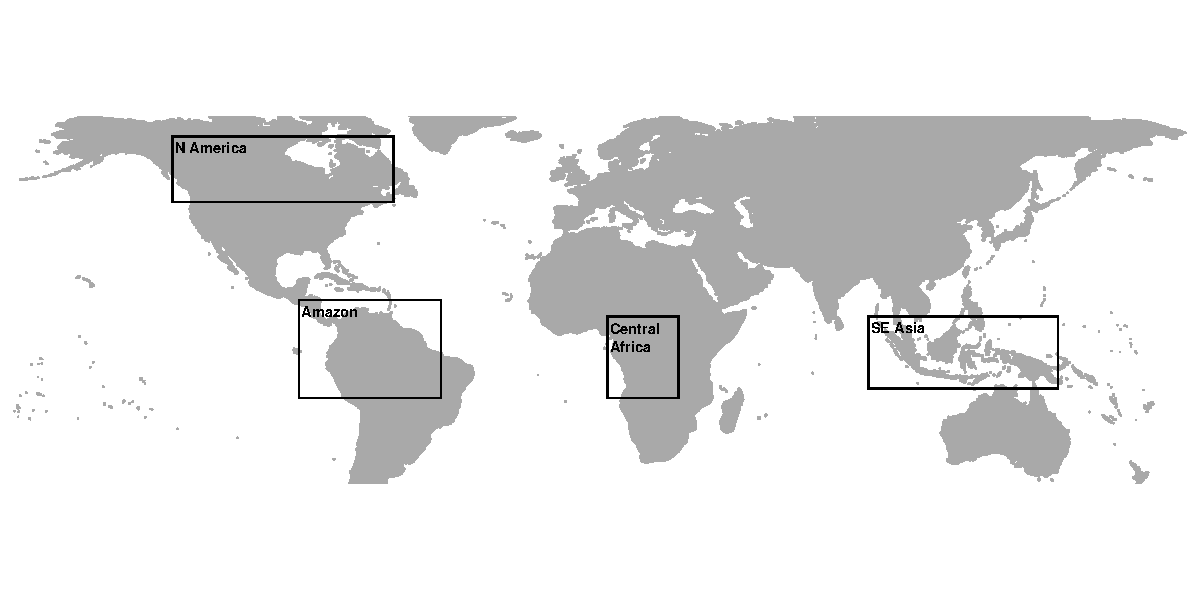
\includegraphics[width=12cm]{graphics/map_forests.pdf}
\caption{A map of the forest regions used in the study. Regions are: Amazon 15\textdegree S - 15\textdegree N, 270\textdegree E - 315\textdegree E; Central Africa; 15\textdegree S - 10\textdegree N, 7.5\textdegree E - 30\textdegree E; SE Asia 12\textdegree S - 10\textdegree N, 90\textdegree E - 150\textdegree E; North America 45\textdegree N - 65\textdegree N, 230\textdegree E - 300\textdegree E.}
\label{fig:map_forests}
\end{figure}

\begin{figure}[t]
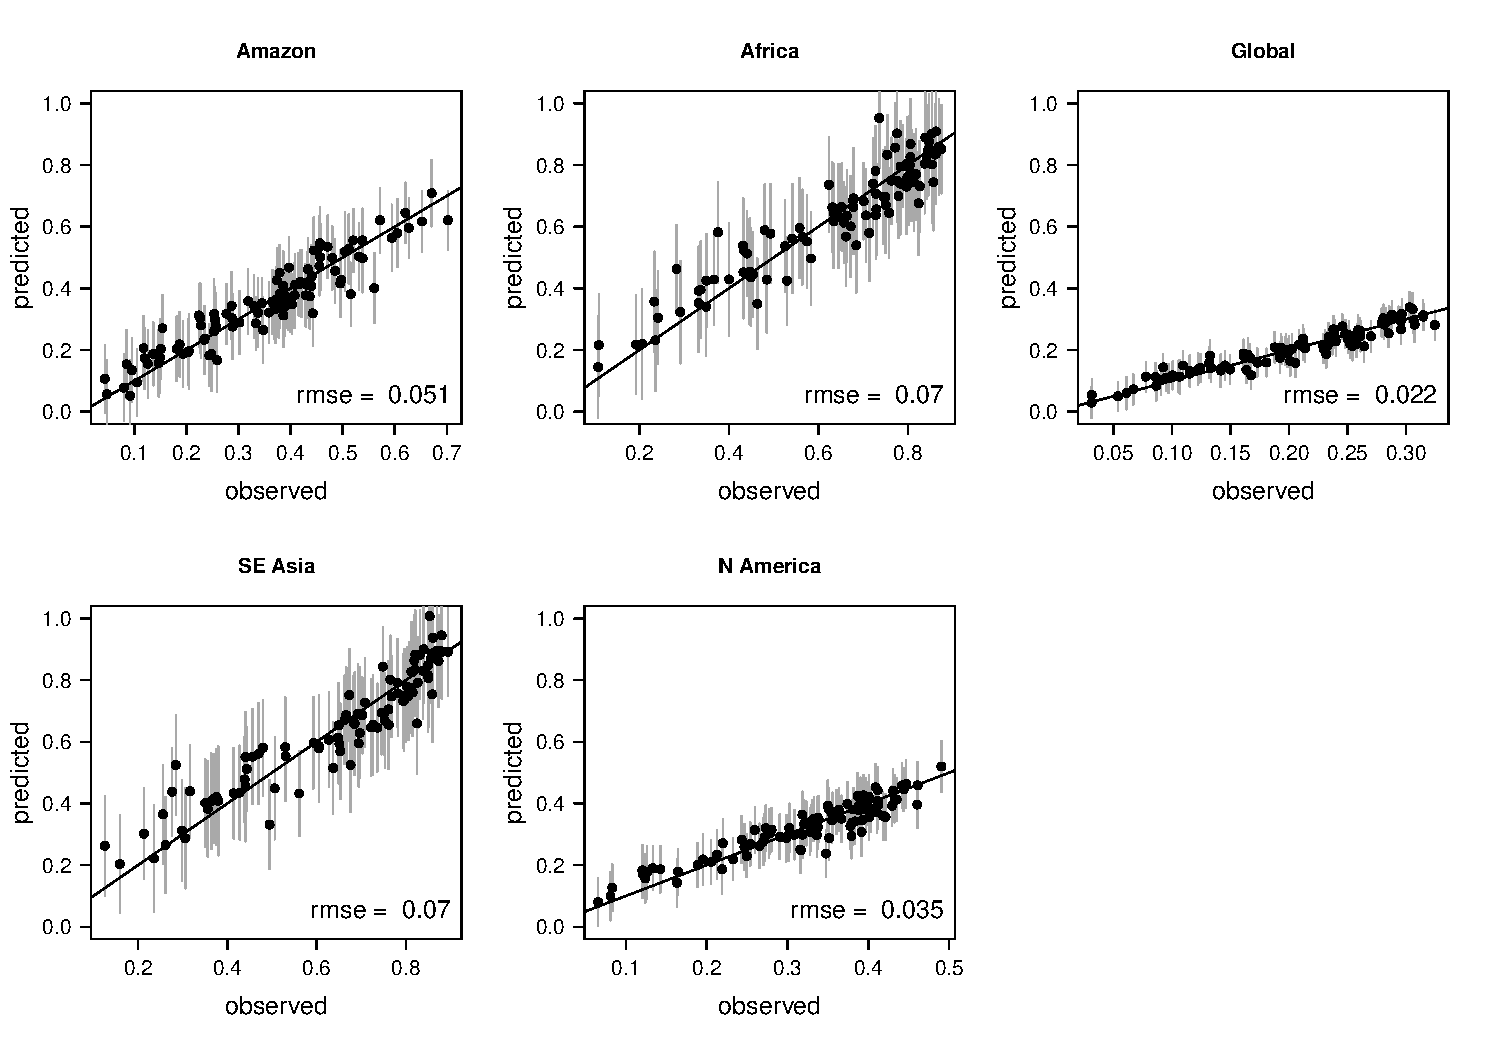
\includegraphics[width=12cm]{graphics/frac_loo.pdf}
\caption{Leave-one-out cross validation performance of the emulator, when reproducing each forest fraction. Black points represent the emulator central estimate of a held-out point, with grey lines representing $\pm$ 2 standard deviations.}
\label{fig:frac_loo}
\end{figure}

\end{document}